% IEEE-style conference layout built on the standard article class (IEEEtran.cls was not available
% in the build environment).  To use the official class, replace the preamble with
%   \documentclass[conference]{IEEEtran}  and move the author block to \IEEEauthorblockN/A.
\documentclass[10pt,twocolumn,letterpaper]{article}
\usepackage[top=0.75in,bottom=1in,left=0.625in,right=0.625in,columnsep=0.25in]{geometry}
\usepackage{mathptmx}
\usepackage[T1]{fontenc}
\usepackage{amsmath,amssymb}
\usepackage{graphicx}
\usepackage{booktabs}
\usepackage{cite}
\usepackage{listings}
\usepackage{tikz}
\usetikzlibrary{shapes.geometric,arrows.meta,positioning,calc}
\usepackage[font=footnotesize,labelfont=bf]{caption}
\usepackage{titlesec}
\usepackage{balance}
\usepackage[hidelinks]{hyperref}
\graphicspath{{../results/figures/}{../../results/figures/}}
\newcommand{\SZeromorMean}{10.0}
\newcommand{\SZeromorPnf}{24.0}
\newcommand{\SZeromorQ}{422}
\newcommand{\SZeromorMov}{43}
\newcommand{\SZeromorLf}{93}
\newcommand{\SZeromorMax}{26.8}
\newcommand{\SZeromorGt}{23}
\newcommand{\SZeromorDen}{65}
\newcommand{\SOnemorMean}{2.4}
\newcommand{\SOnemorPnf}{5.6}
\newcommand{\SOnemorQ}{153}
\newcommand{\SOnemorMov}{55}
\newcommand{\SOnemorLf}{79}
\newcommand{\SOnemorMax}{6.8}
\newcommand{\SOnemorGt}{1}
\newcommand{\SOnemorDen}{28}
\newcommand{\STwomorMean}{2.1}
\newcommand{\STwomorPnf}{5.7}
\newcommand{\STwomorQ}{138}
\newcommand{\STwomorMov}{50}
\newcommand{\STwomorLf}{81}
\newcommand{\STwomorMax}{7.7}
\newcommand{\STwomorGt}{2}
\newcommand{\STwomorDen}{10}
\newcommand{\SThreemorMean}{1.6}
\newcommand{\SThreemorPnf}{4.2}
\newcommand{\SThreemorQ}{123}
\newcommand{\SThreemorMov}{52}
\newcommand{\SThreemorLf}{80}
\newcommand{\SThreemorMax}{6.1}
\newcommand{\SThreemorGt}{0}
\newcommand{\SThreemorDen}{8}
\newcommand{\SFourmorMean}{1.1}
\newcommand{\SFourmorPnf}{2.3}
\newcommand{\SFourmorQ}{67}
\newcommand{\SFourmorMov}{68}
\newcommand{\SFourmorLf}{61}
\newcommand{\SFourmorMax}{6.3}
\newcommand{\SFourmorGt}{0}
\newcommand{\SFourmorDen}{2}
\newcommand{\SOnemorRed}{75}
\newcommand{\SOnemorDci}{1.6}
\newcommand{\SOnemorDdiff}{7.5}
\newcommand{\STwomorRed}{79}
\newcommand{\STwomorDci}{1.6}
\newcommand{\STwomorDdiff}{7.9}
\newcommand{\SThreemorRed}{84}
\newcommand{\SThreemorDci}{1.9}
\newcommand{\SThreemorDdiff}{8.4}
\newcommand{\SFourmorRed}{89}
\newcommand{\SFourmorDci}{2.1}
\newcommand{\SFourmorDdiff}{8.9}
\newcommand{\SZeroaftMean}{15.3}
\newcommand{\SZeroaftPnf}{32.8}
\newcommand{\SZeroaftQ}{550}
\newcommand{\SZeroaftMov}{43}
\newcommand{\SZeroaftLf}{95}
\newcommand{\SZeroaftMax}{35.9}
\newcommand{\SZeroaftGt}{40}
\newcommand{\SZeroaftDen}{80}
\newcommand{\SOneaftMean}{3.9}
\newcommand{\SOneaftPnf}{7.5}
\newcommand{\SOneaftQ}{206}
\newcommand{\SOneaftMov}{55}
\newcommand{\SOneaftLf}{82}
\newcommand{\SOneaftMax}{9.2}
\newcommand{\SOneaftGt}{3}
\newcommand{\SOneaftDen}{45}
\newcommand{\STwoaftMean}{2.8}
\newcommand{\STwoaftPnf}{8.0}
\newcommand{\STwoaftQ}{195}
\newcommand{\STwoaftMov}{51}
\newcommand{\STwoaftLf}{84}
\newcommand{\STwoaftMax}{10.5}
\newcommand{\STwoaftGt}{4}
\newcommand{\STwoaftDen}{16}
\newcommand{\SThreeaftMean}{1.3}
\newcommand{\SThreeaftPnf}{2.8}
\newcommand{\SThreeaftQ}{69}
\newcommand{\SThreeaftMov}{55}
\newcommand{\SThreeaftLf}{81}
\newcommand{\SThreeaftMax}{4.4}
\newcommand{\SThreeaftGt}{0}
\newcommand{\SThreeaftDen}{2}
\newcommand{\SFouraftMean}{1.1}
\newcommand{\SFouraftPnf}{2.5}
\newcommand{\SFouraftQ}{71}
\newcommand{\SFouraftMov}{68}
\newcommand{\SFouraftLf}{63}
\newcommand{\SFouraftMax}{7.1}
\newcommand{\SFouraftGt}{0}
\newcommand{\SFouraftDen}{2}
\newcommand{\SOneaftRed}{75}
\newcommand{\SOneaftDci}{1.7}
\newcommand{\SOneaftDdiff}{11.4}
\newcommand{\STwoaftRed}{81}
\newcommand{\STwoaftDci}{2.0}
\newcommand{\STwoaftDdiff}{12.5}
\newcommand{\SThreeaftRed}{92}
\newcommand{\SThreeaftDci}{2.8}
\newcommand{\SThreeaftDdiff}{14.0}
\newcommand{\SFouraftRed}{93}
\newcommand{\SFouraftDci}{2.8}
\newcommand{\SFouraftDdiff}{14.2}
\newcommand{\eqSZero}{38}
\newcommand{\eqSOne}{28}
\newcommand{\eqSThree}{24}
\newcommand{\eqSFour}{26}
\newcommand{\eqRef}{12.3}
\newcommand{\fourHold}{1}
\newcommand{\fourLoad}{1}
\newcommand{\fourReb}{50}
\newcommand{\repsFinal}{30}
\newcommand{\repsTrain}{10}
\newcommand{\repsSens}{20}
\newcommand{\demSZeroPnf}{58.7}
\newcommand{\demSOnePnf}{17.8}
\newcommand{\demSThreePnf}{7.0}
\newcommand{\demSFourPnf}{4.9}
\newcommand{\hTwoMean}{3.7}
\newcommand{\hThreeMean}{27.3}
\newcommand{\fleetFlat}{12.3}


\titleformat{\section}{\centering\normalfont\small\scshape}{\thesection.}{0.5em}{}
\titleformat{\subsection}{\normalfont\small\itshape}{\thesubsection}{0.5em}{}
\titlespacing*{\section}{0pt}{8pt}{4pt}
\titlespacing*{\subsection}{0pt}{5pt}{2pt}
\renewcommand{\thesection}{\Roman{section}}
\renewcommand{\thesubsection}{\thesection-\Alph{subsection}.}
\setlength{\parskip}{0pt}
\lstset{basicstyle=\ttfamily\scriptsize,frame=single,breaklines=true,columns=fullflexible,
  keywordstyle=\bfseries,numbers=none,xleftmargin=2pt,xrightmargin=2pt,aboveskip=3pt,belowskip=3pt}
\pagestyle{plain}

\begin{document}
\begin{titlepage}
\centering
\vspace*{0.3in}

\includegraphics[width=2.2in]{muet_logo.png}\\[0.3in]
{\Large\bfseries Mehran University of Engineering and Technology\\[2pt] Jamshoro, Sindh, Pakistan}\\[0.15in]
{\large Department of Software Engineering}\\[0.6in]
{\large Project-Based Learning (PBL) Assignment}\\[0.3in]
\rule{\textwidth}{0.8pt}\\[0.2in]
{\LARGE\bfseries Modeling, Simulation and Scheduling Optimization\\[4pt] of the MUET Point Bus System}\\[0.2in]
\rule{\textwidth}{0.8pt}\\[0.6in]
{\large\bfseries Submitted by}\\[0.15in]
\begin{tabular}{rl}
\large Name: & \large Sumit Sharma\\[4pt]
\large Roll Number: & \large 22SW027\\[4pt]
\large Section: & \large 3\\
\end{tabular}\\[0.6in]
{\large November 25, 2026}
\end{titlepage}
\setcounter{page}{1}

\title{\vspace{-0.4in}\Large\bfseries Modeling, Simulation and Scheduling Optimization of the\\ MUET Point Bus System}
\author{\normalsize Sumit Sharma (22SW027, Section 3)\\
\small Department of Software Engineering, Mehran University of Engineering and Technology, Jamshoro, Pakistan\\
}
\date{}
\maketitle
\vspace{-0.3in}

\begin{abstract}
Mehran University's Point buses carry thousands of students daily between Hyderabad and Jamshoro, yet
students queue for long periods at the STC and Main Gate terminals during the 08:00--09:00 and
14:00--15:30 peaks. We build a discrete-event simulation (DES) of the two-terminal bus loop,
with non-homogeneous Poisson passenger arrivals, stochastic trip times and a fixed fleet of 40 buses, and use it to
diagnose the bottleneck and to test dispatch strategies \emph{without purchasing buses}. A static
timetable with a 2.5\,min peak headway (the assumed baseline) yields a mean wait of \SZeromorMean\,min
(morning) and \SZeroaftMean\,min (afternoon) with 95th-percentile waits of \SZeromorPnf--\SZeroaftPnf\,min, because its
capacity ($\approx$20 pax/min) is below peak demand ($\approx$25 pax/min) while about half the fleet sits idle in terminal
lines. A simple demand-responsive ``full-load-or-short-hold'' dispatch rule, tuned by simulation-based grid search,
cuts the mean wait by \SFourmorRed\% and \SFouraftRed\%, and matches the baseline's mean wait with
only \eqSFour{} buses instead of 40 (30 replications, common random numbers, 95\% CIs). \emph{All demand and trip-time inputs are
assumptions, not MUET measurements}; the framework is built to be re-calibrated with field data.
\end{abstract}

\noindent\textbf{Keywords:} discrete-event simulation, queueing theory, bus dispatching, holding control, what-if analysis.

%--------------------------------------------------------------------
\section{Introduction}
The MUET transport administration relies on a dedicated Point fleet to move students, faculty and staff
between Hyderabad and the Jamshoro campus. Peak-hour symptoms reported by the administration are long waits at the STC and
Main Gate terminals, over-capacity buses, and a static schedule that cannot react to varying loads or traffic delays. This
report answers two questions: \emph{(i)} how can the existing scheduling and queue-management system be modeled, simulated and
analyzed to identify bottlenecks, and \emph{(ii)} which algorithmic scheduling optimizations minimize waiting time and maximize
fleet utilization with the current fleet?

Contributions: (1) a conceptual model (state-transition diagrams and flowchart); (2) a mathematical model combining
non-homogeneous Poisson arrivals, bulk-service boarding, stochastic cycle times and a fluid capacity balance; (3) a verified
Python DES with common random numbers; (4) a bottleneck diagnosis of a static timetable; (5) four scheduling scenarios plus a
tuned policy, evaluated by what-if and sensitivity analysis; (6) implementation recommendations.

\section{System Description and Assumptions}
\subsection{System}
The system is a closed loop of $N$ buses between terminal A (STC, Hyderabad) and terminal B (Main Gate, Jamshoro).
Demand is strongly directional: A$\to$B dominates in the morning, B$\to$A in the afternoon
(Fig.~\ref{fig:demand}). Each terminal has one boarding bay, a FIFO passenger queue, and a FIFO line of waiting buses.

\subsection{Data status and assumptions}
\textbf{No measured MUET data were available.} Table~\ref{tab:params} lists the assumed inputs. They were chosen to be
plausible and so that the baseline reproduces the reported symptoms (peak waits of 15+ min and over-full buses); the
\emph{absolute} numbers therefore must not be read as MUET measurements. What the study does support are the \emph{relative} comparisons and the
mechanisms. The code accepts observed demand profiles (CSV) for calibration.

\begin{table}[t]
\centering\caption{Assumed model parameters (all to be replaced by field data).}\label{tab:params}
\footnotesize
\begin{tabular}{@{}lp{0.6\columnwidth}@{}}\toprule
Fleet $N$ / capacity $C$ & 40 buses / 50 pax (seated + standing)\\
One-way trip time & mean 25 min, CV 0.18; $\times1.15$ in peak; incident prob.\ 0.04, mean 8 min\\
Alighting + layover & 1 min + 2 min\\
Boarding time & 0.5 min + 0.8 s per passenger, one bay per terminal\\
Peak demand (dominant dir.) & $\approx$25--26 pax/min; $\approx$2.9k--3.3k pax per 3-h window\\
Opposite direction & 2.5 pax/min\\
Day-to-day variation & demand CV 12\%, road-condition CV 8\%\\
Baseline timetable & headway 2.5 min (07:30--09:30 / 14:00--16:00), 5 min otherwise\\
\bottomrule\end{tabular}
\end{table}

\begin{figure}[t]\centering
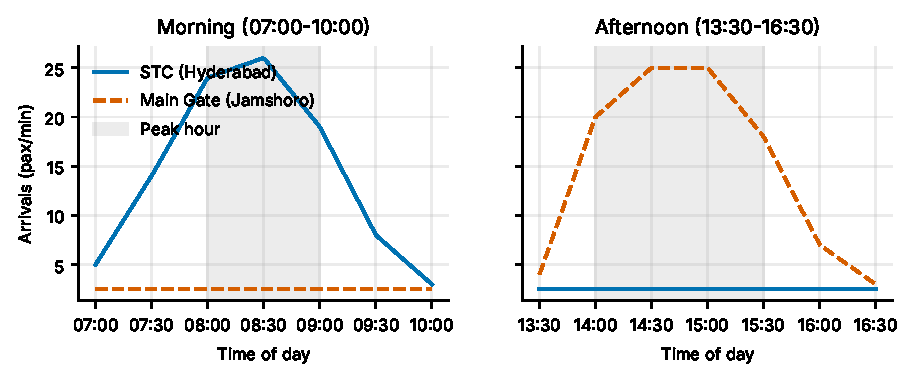
\includegraphics[width=\columnwidth]{fig_demand}
\caption{Assumed passenger arrival-rate profiles $\lambda(t)$; shaded = peak hour(s).}\label{fig:demand}
\end{figure}

\section{Conceptual Model}
Fig.~\ref{fig:states} shows the state-transition diagrams of a bus and of a passenger; Fig.~\ref{fig:flow} the dispatch decision
logic evaluated for the bus in the bay.

\begin{figure}[t]\centering
\resizebox{\columnwidth}{!}{%
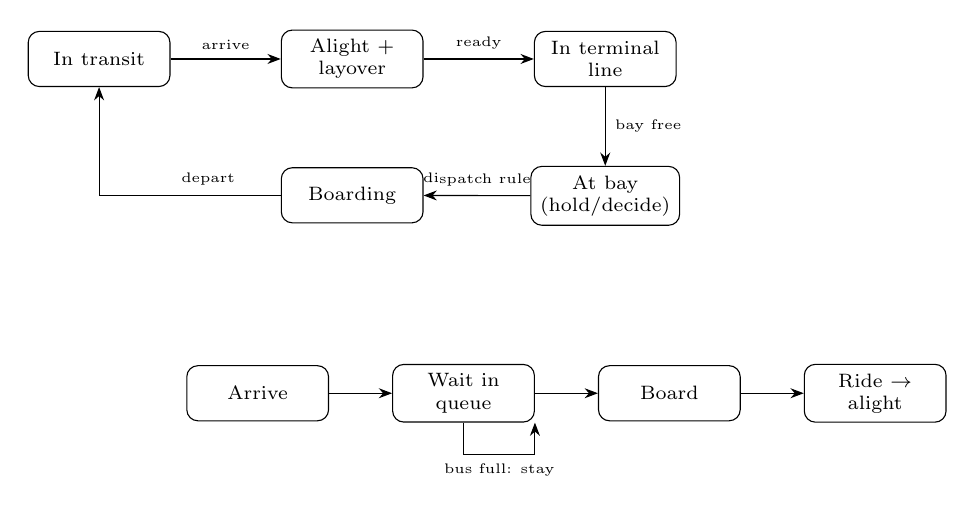
\begin{tikzpicture}[>=Stealth,node distance=10mm,
 st/.style={draw,rounded corners,minimum width=18mm,minimum height=7mm,font=\scriptsize,align=center},
 lab/.style={font=\tiny,midway,above,sloped}]
\node[st] (tr) {In transit};
\node[st,right=14mm of tr] (al) {Alight +\\layover};
\node[st,right=14mm of al] (ln) {In terminal\\line};
\node[st,below=10mm of ln] (bay) {At bay\\(hold/decide)};
\node[st,below=10mm of al] (bd) {Boarding};
\draw[->] (tr) -- node[lab]{arrive} (al);
\draw[->] (al) -- node[lab]{ready} (ln);
\draw[->] (ln) -- node[lab,right,sloped=false]{bay free} (bay);
\draw[->] (bay) -- node[lab]{dispatch rule} (bd);
\draw[->] (bd) -| node[lab,pos=0.2]{depart} (tr);
% passenger chain
\node[st,below=18mm of bd,xshift=-12mm] (p1) {Arrive};
\node[st,right=8mm of p1] (p2) {Wait in\\queue};
\node[st,right=8mm of p2] (p3) {Board};
\node[st,right=8mm of p3] (p4) {Ride $\to$\\alight};
\draw[->] (p1) -- (p2); \draw[->] (p2) -- (p3); \draw[->] (p3) -- (p4);
\draw[->] (p2.south) -- ++(0,-4mm) -| node[font=\tiny,pos=0.25,below]{bus full: stay} (p2.south east);
\end{tikzpicture}}
\caption{State-transition diagrams: bus (top) and passenger (bottom).}\label{fig:states}
\end{figure}

\begin{figure}[t]\centering
\resizebox{0.92\columnwidth}{!}{%
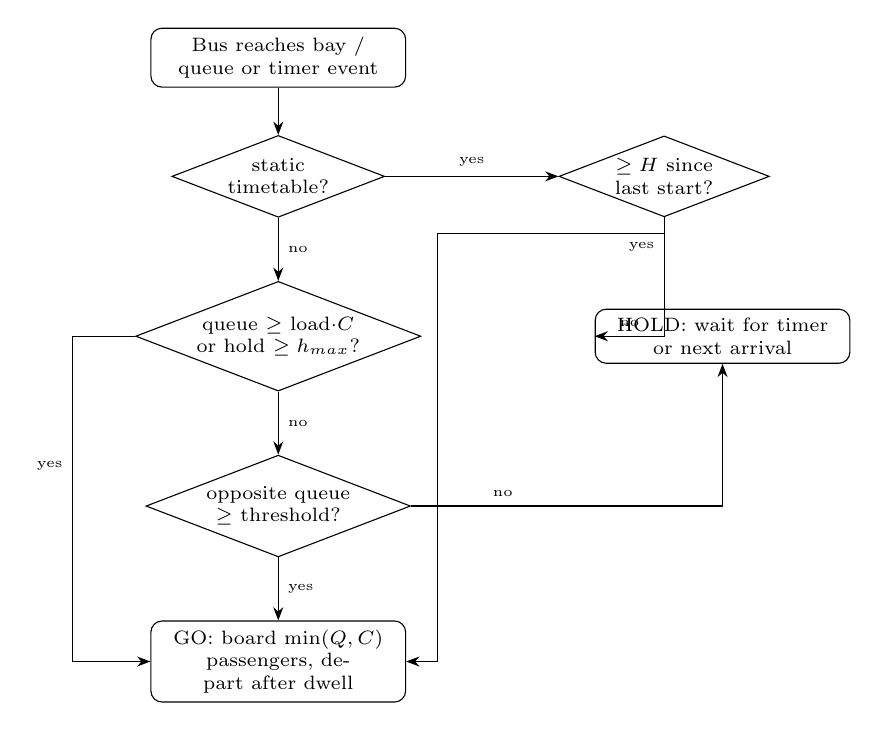
\begin{tikzpicture}[>=Stealth,node distance=6mm,
 pr/.style={draw,rectangle,rounded corners,font=\scriptsize,align=center,minimum height=6mm,text width=30mm},
 dc/.style={draw,diamond,aspect=2.6,font=\scriptsize,align=center,inner sep=1pt}]
\node[pr] (a) {Bus reaches bay / queue or timer event};
\node[dc,below=of a] (k) {static\\timetable?};
\node[dc,right=22mm of k] (h) {$\ge H$ since\\last start?};
\node[dc,below=8mm of k] (f) {queue $\ge$ load$\cdot C$\\or hold $\ge h_{max}$?};
\node[dc,below=8mm of f] (r) {opposite queue\\$\ge$ threshold?};
\node[pr,below=8mm of r] (g) {GO: board $\min(Q,C)$\\passengers, depart after dwell};
\node[pr,right=22mm of f] (w) {HOLD: wait for timer\\or next arrival};
\draw[->] (a)--(k);
\draw[->] (k)--node[above,font=\tiny]{yes}(h);
\draw[->] (k)--node[right,font=\tiny]{no}(f);
\draw[->] (h) |- node[above,font=\tiny,pos=0.75]{no} (w);
\draw[->] (f)--node[right,font=\tiny]{no}(r);
\draw[->] (r)--node[right,font=\tiny]{yes}(g);
\draw[->] (f.west) -- ++(-8mm,0) |- node[left,font=\tiny,pos=0.2]{yes} (g.west);
\draw[->] (r.east) -- node[above,font=\tiny]{no} (w.south west|-r.east) -| (w);
\draw[->] (h.south) -- ++(0,-2mm) -| node[font=\tiny,pos=0.05,below]{yes} ($(g.east)+(4mm,0)$) -- (g.east);
\end{tikzpicture}}
\caption{Dispatch decision flowchart (static and dynamic policies).}\label{fig:flow}
\end{figure}

\section{Mathematical Model}
\subsection{Passenger arrivals}
Arrivals at terminal $k$ follow a non-homogeneous Poisson process with piecewise-linear rate $\lambda_k(t)$,
scaled by a day factor $F_d$ (lognormal, mean 1). Samples are generated by thinning \cite{law}: draw $n\sim\text{Poisson}(\lambda_{max}T)$
candidates uniformly on $[0,T]$ and keep each with probability $\lambda_k(t)/\lambda_{max}$. Expected demand is $\Lambda=\int_0^T\lambda_k(t)\,dt$.

\subsection{Boarding and trips}
When boarding starts at time $t$ with $Q$ passengers waiting, $n=\min(Q,C)$ board in FIFO order, wait $W_i=t-a_i$, and the bay is
busy for $d=d_0+d_1 n$. A trip takes
\begin{equation}
T_{trip}=F_r\,m(t)\,e^{\sigma Z-\sigma^2/2}+B\,E,\quad \sigma^2=\ln(1+\mathrm{CV}^2),
\end{equation}
with $Z\sim N(0,1)$, $B\sim\text{Bernoulli}(p)$, $E\sim\text{Exp}(\mu_{inc})$, road factor $F_r$ and $m(t)$ the mean (raised by 15\% in peak).

\subsection{Capacity, utilization and fluid queue}
The cycle time of a bus is $T_c=2\bar\tau+2(a+l)+d_A+d_B+h$ ($\bar\tau$ mean trip, $a,l$ alighting and layover, $h$ holding).
A fleet can therefore supply at most
\begin{equation}
\mu_{fleet}=\frac{N\,C}{T_c}\ \text{pax/min},\qquad \mu_{static}=\min\!\Big(\frac{C}{H},\mu_{fleet}\Big),
\end{equation}
and the peak utilization is $\rho=\lambda_{pk}/\mu$. The deterministic queue obeys
$\dot Q=\lambda(t)-\mu(t)$ while $Q>0$ \cite{kleinrock}. With $C=50$, $H=2.5$ min, $\mu_{static}=20$ pax/min while $\mu_{fleet}\approx30$
pax/min: the timetable, not the fleet, limits capacity.

\subsection{Performance measures}
Mean wait $\bar W=\frac1n\sum W_i$; $P_{95}$; share waiting $>15$ min; peak queue; \emph{fleet-in-motion share}
$\sum T_{trip}/(N\,T_{end})$ (utilization of the fleet in service); \emph{load factor} $=\sum n/(C\cdot\#\text{trips})$. Little's law
$L=\lambda_{eff}\bar W$ holds exactly per run, which we use as a test \cite{little}. Confidence intervals use the $t$ distribution over
independent replications; policy differences are \emph{paired} on common random numbers \cite{law,banks}.

\subsection{Policies}
\textbf{Static}: a bus may start boarding only if at least $H(t)$ min elapsed since the previous start. \textbf{Dynamic hold-and-go}
(related to holding control \cite{osuna}): the bay bus departs when the queue reaches a load threshold $\ell C$ ($\ell=1$: full), or after holding $h_{max}$ min,
or---with rebalancing---when the opposite queue exceeds $\theta$ passengers (deadhead immediately toward the loaded end).
Parameters $(h_{max},\ell,\theta)$ are chosen by grid search minimizing $J=\overline{\bar W+0.5P_{95}}$ over nominal and $+25\%$ demand on training seeds disjoint from the
test seeds. Scenarios: S0 baseline timetable; S1 denser timetable (2.0/4.0 min); S2 dynamic ($h_{max}=2,\ell=1$); S3 S2 + rebalancing ($\theta=50$);
S4 tuned ($h_{max}=\fourHold$, $\ell=\fourLoad$, $\theta=$\,\fourReb).

\section{Simulation Implementation}
The model is Python 3 with a custom event-calendar kernel (SimPy was not installable offline; the kernel is 30 lines).
Modules: \texttt{des.py} (kernel), \texttt{model.py} (bus system), \texttt{config.py}, \texttt{fluid.py},
\texttt{run\_experiments.py}, \texttt{make\_figures.py}, \texttt{test\_model.py}. Random inputs (arrivals, per-bus per-trip variates) depend only on the seed (common
random numbers).

\begin{lstlisting}[language=Python,caption={Event kernel (des.py).}]
class Simulator:
    def schedule(self, delay, fn, *args):
        heapq.heappush(self._heap,
            (self.now + delay, next(self._seq), fn, args))
    def run(self, until=inf, stop=None):
        while self._heap and self._heap[0][0] <= until:
            t, _, fn, args = heapq.heappop(self._heap)
            self.now = t; fn(*args)
            if stop and stop(): break
\end{lstlisting}

\begin{lstlisting}[language=Python,caption={Dynamic dispatch decision (model.py).}]
n = len(term.queue); other = self.terms[1 - term.idx]
held = now - term.front_ready
go = (n >= cap or n >= pol.min_load * cap
      or held >= pol.max_hold
      or (pol.rebal_thr is not None
          and len(other.queue) >= pol.rebal_thr))
if go: self._go(term)
\end{lstlisting}

\begin{lstlisting}[language=Python,caption={Non-homogeneous Poisson arrivals by thinning.}]
n = rng.poisson(lam_max * horizon)
cand = np.sort(rng.uniform(0, horizon, n))
u = rng.uniform(0, lam_max, n)
return cand[u < scale * np.interp(cand, xs, ys)]
\end{lstlisting}

\section{Verification and Validation}
Nine automated tests pass (\texttt{python -m unittest}): (i) passengers and buses are conserved and no bus exceeds capacity; (ii)
the integral of queue length equals the sum of individual waits (Little's law identity, tolerance $10^{-6}$); (iii) with uniform arrivals and ample
buses a fixed headway $H$ gives mean wait $H/2$ (analytic check within 0.08 min); (iv) expected arrivals match $\Lambda$; (v) common
random numbers give identical demand across policies and reproducible runs; (vi) static headway and full-load dispatch behave as specified.

Table~\ref{tab:fluid} compares the fluid model with the simulation. The fluid model correctly flags the baseline as over-saturated
($\rho_{pk}>1$) and the dynamic policies as under-saturated, and gets the order of magnitude of the baseline queue, but it underestimates peak queues because it ignores
stochastic variation and the batch (full-bus) nature of service; for dynamic policies it predicts essentially no queue whereas the simulation shows 1--2 busloads.
\emph{Validation against real MUET data has not been done}: without field data the model is verified, not validated.

\begin{table}[t]\centering\caption{Fluid approximation vs.\ simulation (peak queue at dominant terminal, passengers).}\label{tab:fluid}
\footnotesize\begin{tabular}{@{}llccccc@{}}\toprule
Period & Scen. & $\rho_{pk}$ & Fluid $Q_{max}$ & Fluid (day-avg) & Sim. $Q_{max}$ \\ \midrule
Mor. & S0 & 1.30 & 251 & 280 & 422$\pm$71 \\
Mor. & S1 & 1.04 & 10 & 54 & 153$\pm$37 \\
Mor. & S3 & 0.86 & 0 & 3 & 123$\pm$42 \\
Mor. & S4 & 0.86 & 0 & 3 & 67$\pm$25 \\
Aft. & S0 & 1.25 & 372 & 389 & 550$\pm$84 \\
Aft. & S1 & 1.00 & 53 & 100 & 206$\pm$53 \\
Aft. & S3 & 0.82 & 0 & 2 & 69$\pm$25 \\
Aft. & S4 & 0.82 & 0 & 2 & 71$\pm$29 \\
\bottomrule\end{tabular}

\end{table}

\section{Baseline Analysis and Bottlenecks}
\begin{figure}[t]\centering
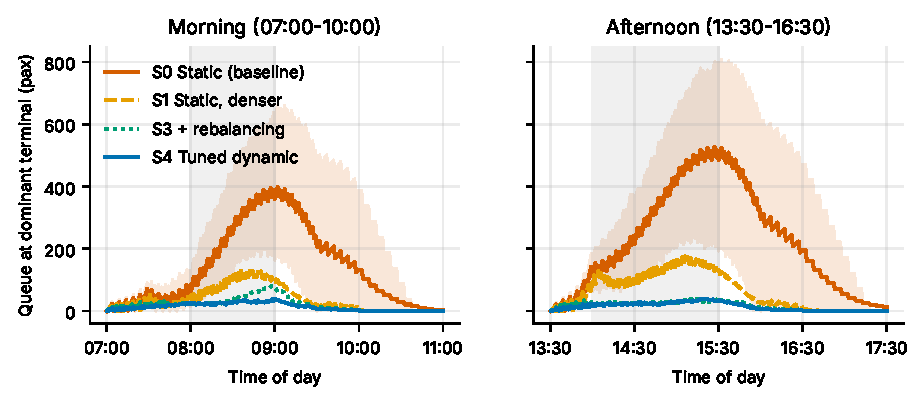
\includegraphics[width=\columnwidth]{fig_queue}
\caption{Mean queue at the dominant terminal (30 replications); band = 10--90\% of S0.}\label{fig:queue}
\end{figure}
Under S0 the queue grows through the peak to about \SZeromorQ{} (morning) and \SZeroaftQ{} (afternoon) passengers (Fig.~\ref{fig:queue}), and \SZeromorDen\%/\SZeroaftDen\%
of passengers are left behind by at least one full bus. Buses depart \SZeromorLf--\SZeroaftLf\% full. Three findings identify the bottleneck:
\begin{enumerate}
\item \emph{Capacity gap, not fleet shortage.} $\rho_{pk}=1.25$--$1.30$ for the timetable. Adding buses does not help: S0's mean wait stays at
$\approx$\fleetFlat\,min for any fleet size above 34 (Fig.~\ref{fig:sens}, left), because the headway caps departures.
\item \emph{Idle buses while passengers wait.} Only \SZeromorMov\% of fleet time is in motion; the rest is spent in terminal lines and layovers, held for the next timetable slot.
\item \emph{Brittleness.} A static headway is a knife edge: peak headway 2.0\,min gives \hTwoMean\,min mean wait, 3.0\,min gives \hThreeMean\,min
(Fig.~\ref{fig:sens}, right). Boarding bays are not limiting (utilization about 50\% or less).
\end{enumerate}

\section{Scenario (What-If) Results}
\begin{table}[t]\centering\caption{Morning window (mean$\pm$95\% CI over \repsFinal{} replications).}\label{tab:mor}
\footnotesize\setlength{\tabcolsep}{2.5pt}\begin{tabular}{@{}lccccc@{}}\toprule
Metric & S0 & S1 & S2 & S3 & S4 \\ \midrule
Mean wait (min) & 10.0$\pm$2.2 & 2.4$\pm$0.6 & 2.1$\pm$0.7 & 1.6$\pm$0.3 & 1.1$\pm$0.2 \\
P95 wait (min) & 24.0$\pm$6.3 & 5.6$\pm$1.4 & 5.7$\pm$2.4 & 4.2$\pm$1.2 & 2.3$\pm$0.7 \\
Max wait (min) & 26.8 & 6.8 & 7.7 & 6.1 & 6.3 \\
Wait $>$15 min (\%) & 23.2 & 0.9 & 2.1 & 0.2 & 0.0 \\
Peak queue (pax) & 422 & 153 & 138 & 123 & 67 \\
Left behind (\%) & 65 & 28 & 10 & 8 & 2 \\
Fleet in motion (\%) & 43 & 55 & 50 & 52 & 68 \\
Load factor, dom. dir. (\%) & 93 & 79 & 81 & 80 & 61 \\
\bottomrule\end{tabular}

\end{table}
\begin{table}[t]\centering\caption{Afternoon window (mean$\pm$95\% CI over \repsFinal{} replications).}\label{tab:aft}
\footnotesize\setlength{\tabcolsep}{2.5pt}\begin{tabular}{@{}lccccc@{}}\toprule
Metric & S0 & S1 & S2 & S3 & S4 \\ \midrule
Mean wait (min) & 15.3$\pm$2.9 & 3.9$\pm$1.2 & 2.8$\pm$1.1 & 1.3$\pm$0.2 & 1.1$\pm$0.2 \\
P95 wait (min) & 32.8$\pm$7.8 & 7.5$\pm$2.2 & 8.0$\pm$3.3 & 2.8$\pm$0.7 & 2.5$\pm$0.9 \\
Max wait (min) & 35.9 & 9.2 & 10.5 & 4.4 & 7.1 \\
Wait $>$15 min (\%) & 40.2 & 3.1 & 3.8 & 0.0 & 0.1 \\
Peak queue (pax) & 550 & 206 & 195 & 69 & 71 \\
Left behind (\%) & 80 & 45 & 16 & 2 & 2 \\
Fleet in motion (\%) & 43 & 55 & 51 & 55 & 68 \\
Load factor, dom. dir. (\%) & 95 & 82 & 84 & 81 & 63 \\
\bottomrule\end{tabular}

\end{table}

\begin{figure}[t]\centering
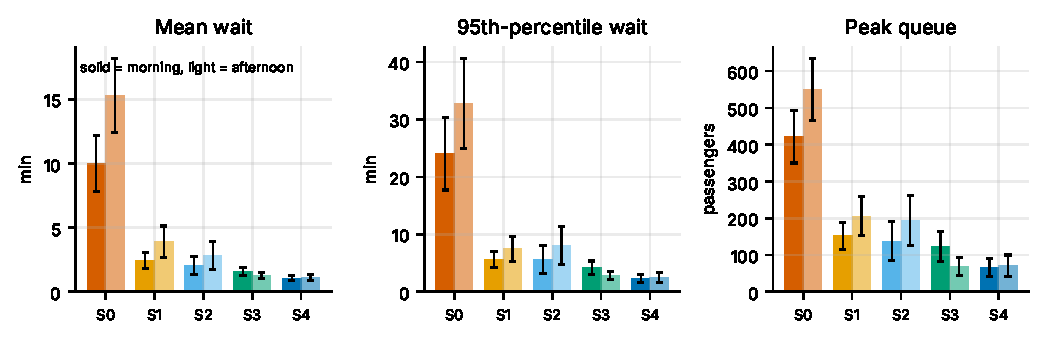
\includegraphics[width=\columnwidth]{fig_metrics}
\caption{Wait and queue metrics by scenario (error bars: 95\% CI).}\label{fig:metrics}
\end{figure}
\begin{figure}[t]\centering
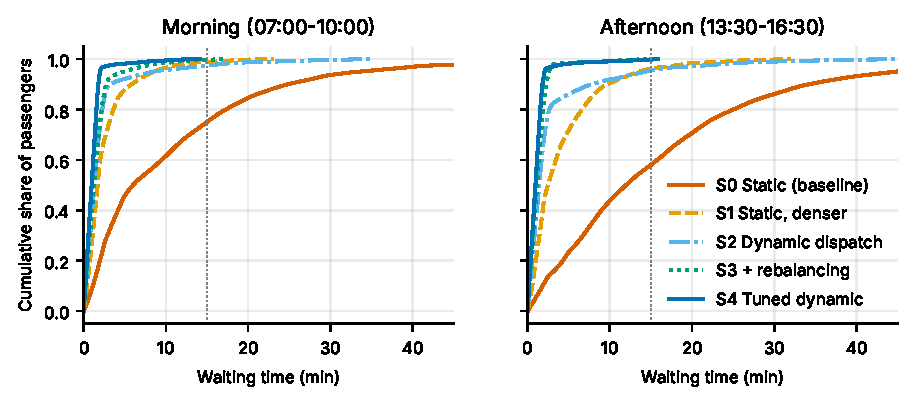
\includegraphics[width=\columnwidth]{fig_wait_cdf}
\caption{Distribution of passenger waiting time (pooled over replications).}\label{fig:cdf}
\end{figure}

Tables~\ref{tab:mor}--\ref{tab:aft} and Figs.~\ref{fig:metrics}--\ref{fig:cdf} summarize the scenarios. Paired reductions of the mean wait relative to S0 are
\SOnemorRed/\SOneaftRed\% (S1), \STwomorRed/\STwoaftRed\% (S2), \SThreemorRed/\SThreeaftRed\% (S3) and \SFourmorRed/\SFouraftRed\% (S4)
(morning/afternoon; S4 paired difference \SFourmorDdiff$\pm$\SFourmorDci\,min morning). Share of passengers waiting over 15 min drops from \SZeromorGt\%/\SZeroaftGt\% to
\SFourmorGt\%/\SFouraftGt\%.
Main reasons: dynamic dispatch removes idle slot-holding at the heavy terminal, and short holds at the light terminal return buses to the loaded end sooner (S2 with 2-min
holds is clearly worse than S4 with \fourHold-min holds, because holding consumes scarce bus-cycles). Rebalancing matters little on nominal days but helps under stress.
Table~\ref{tab:grid} lists the best grid points; the optimum is flat enough that the rule is not fragile.

\begin{table}[t]\centering\caption{Best five grid-search settings (robust objective $J$).}\label{tab:grid}
\footnotesize\begin{tabular}{@{}cccc@{}}\toprule
Hold (min) & Min load & Rebal. thr. & $J$ (min) \\ \midrule
1 & 1 & 50 & 2.26 \\
1 & 1 & 25 & 2.28 \\
1 & 1 & 100 & 2.31 \\
1 & 1 & 200 & 2.33 \\
1 & 1 & off & 2.35 \\
\bottomrule\end{tabular}

\end{table}

\begin{figure}[t]\centering
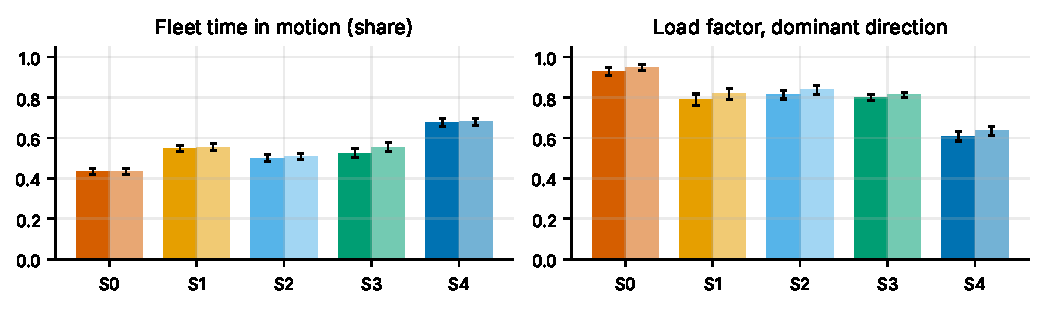
\includegraphics[width=\columnwidth]{fig_util}
\caption{Fleet utilization: share of time in motion (left) and load factor in the dominant direction (right).}\label{fig:util}
\end{figure}
\textbf{Utilization trade-off.} The fraction of fleet time in motion rises from \SZeromorMov\%/\SZeroaftMov\% (S0) to \SFourmorMov\%/\SFouraftMov\% (S4), but the
load factor falls from \SZeromorLf\%/\SZeroaftLf\% to \SFourmorLf\%/\SFouraftLf\%. Buses leave earlier and less crowded: this reduces over-capacity
trips and waiting but means that seat-occupancy ``efficiency'' is lower. We regard this as the intended outcome, but the administration must choose what ``utilization'' means.

\begin{figure*}[t]\centering
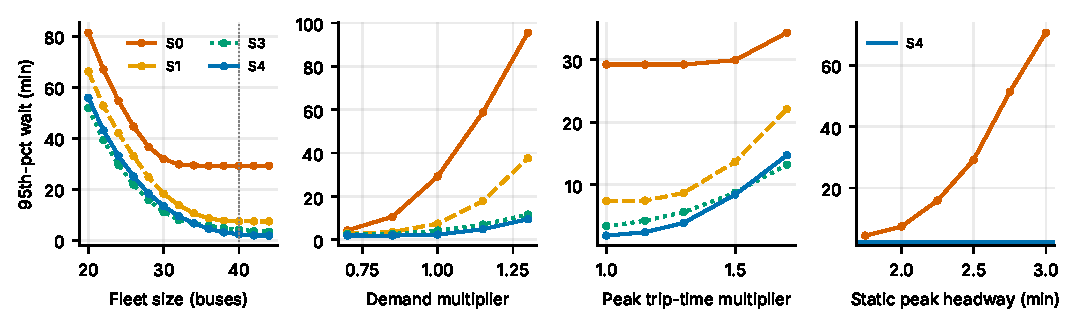
\includegraphics[width=\textwidth]{fig_sensitivity}
\caption{Sensitivity of 95th-percentile wait (avg.\ of both windows) to fleet size, demand level, peak trip-time multiplier, and static headway; S4 is the horizontal line (right).}\label{fig:sens}
\end{figure*}
\textbf{Sensitivity (Fig.~\ref{fig:sens}).} (a) \emph{Fleet size}: with dynamic dispatch the baseline's 40-bus mean wait (\eqRef\,min) is matched with \eqSThree--\eqSFour{} buses
(S3/S4), versus \eqSOne{} for S1 and \eqSZero{} for S0, i.e.\ potential fleet savings of about 35\%, or spare buses for other routes. (b) \emph{Demand}: at $+15\%$ demand the
95th-percentile wait is \demSZeroPnf\,min (S0), \demSOnePnf\,min (S1), \demSThreePnf\,min (S3) and \demSFourPnf\,min (S4). (c) \emph{Traffic}: S0 is insensitive to slower trips
until the fleet becomes limiting, whereas dynamic policies degrade gradually; with peak trip times 70\% longer, S4 and S3 remain far better than S0.

\section{Recommendations}
\begin{enumerate}
\item Replace the fixed timetable by \emph{full-load-or-short-hold} dispatch: a terminal supervisor sends the bay bus when it is full or after at most \fourHold\,min (plus an
immediate departure when the opposite queue exceeds $\approx$50), using visual queue counts or a simple counter/app.
\item Keep holds short (about 1 min). Longer holds consume bus cycles and hurt waiting time.
\item Do not buy buses for the peak: the bottleneck is the timetable. Redeploying the fleet by the dynamic rule gives equal waits with substantially fewer buses; re-evaluate the fleet size
after calibration.
\item Collect data to calibrate: 5-min boarding counts at both terminals, bus GPS or stopwatch trip times, and bus departure logs; then re-run \texttt{run\_experiments.py}.
\item Pilot on one week at one terminal (A/B comparison against the timetable) before a full roll-out.
\end{enumerate}

\section{Limitations and Future Work}
All inputs are assumptions (Table~\ref{tab:params}); the baseline headway was set so that the baseline matches the described symptoms, so the \emph{size} of the improvement
(e.g.\ 90\%) is conditional on that choice and is smaller against a well-tuned static timetable (S1: \SOnemorRed/\SOneaftRed\%). The dynamic policies assume reliable queue
information, driver compliance and no extra intermediate stops; one bay per terminal; no route stops between the two terminals; no individual bus breakdowns; passengers
neither balk nor use other transport. Future work: calibration with field data, multiple routes and bays, predictive holding using forecast demand, and a SimPy/AnyLogic
implementation for cross-validation.

\section{Conclusion}
A verified discrete-event model shows that the MUET Point peak problem is a scheduling problem: a static timetable caps capacity below peak demand while buses idle. A
demand-responsive dispatch rule with short holds removes most of the waiting without additional buses and is robust to demand and traffic variation. These conclusions hold under the stated
assumptions and should be confirmed with measured MUET data.

\section*{Appendix: Reproducing the Results}
\texttt{pip install -r requirements.txt; python -m unittest -v; python run\_experiments.py; python make\_figures.py;} then compile \texttt{report/main.tex} with pdflatex.

\begin{thebibliography}{9}\footnotesize
\bibitem{kleinrock} L. Kleinrock, \emph{Queueing Systems, Vol.\ 1: Theory}. New York: Wiley, 1975.
\bibitem{law} A. M. Law, \emph{Simulation Modeling and Analysis}, 5th ed. New York: McGraw-Hill, 2015.
\bibitem{banks} J. Banks, J. S. Carson II, B. L. Nelson, and D. M. Nicol, \emph{Discrete-Event System Simulation}, 5th ed. Upper Saddle River, NJ: Pearson, 2010.
\bibitem{little} J. D. C. Little, ``A proof for the queuing formula: $L=\lambda W$,'' \emph{Oper.\ Res.}, vol.\ 9, no.\ 3, pp.\ 383--387, 1961.
\bibitem{osuna} E. E. Osuna and G. F. Newell, ``Control strategies for an idealized public transportation system,'' \emph{Transp.\ Sci.}, vol.\ 6, no.\ 1, pp.\ 52--72, 1972.
\end{thebibliography}
\end{document}
